\chapter{Trabalhos Relacionados}

Neste capítulo serão apresentadas três soluções (RiMOM-2015, LogMap e Lily) para o alinhamento de dados conectados. As ferramentas apresentadas a seguir foram selecionadas devido ao seu destaque na edição de 2015 do relatório publicado pela Ontology Alignment Evaluation Initiative (OAEI). Inicialmente, a OAEI avaliava apenas ferramentas de alinhamento de ontologias, dando início à avaliação de soluções para alinhar dados apenas em 2009. Desde então, um número crescente aplicações vêm sendo submetidas.

\section*{RiMOM-2015}
Baseando-se no RiMOM \cite{li2009rimom}, \citeonline{zhang2015rimom} desenvolveram o RiMOM-2015, que é uma ferramenta para alinhar dados conectados. Ela implementa um número considerável de abordagens para alinhar, cuja escolha é realizada através dos metadados extraídos da ontologia. Além disso, o RiMOM-2015 utiliza um índice invertido para indexar os objetos e consequentemente gerar pares candidatos para um possível alinhamento. A geração dos pares é realizada quando dois recursos compartilham pelo menos um predicado e objeto.

Por um lado, o índice invertido permite que um número menor de comparações seja realizado. Por outro lado, a etapa de 
construção desse índice não considera que os objetos indexados podem conter qualquer tipo de erro. Além disso, como pode ser visto na Figura \ref{fig:rimom}, o RiMOM-2015 utiliza as ontologias apenas para alinhar as propriedades e como entrada para a geração de metadados.

\begin{figure}[!ht]
	\centering
	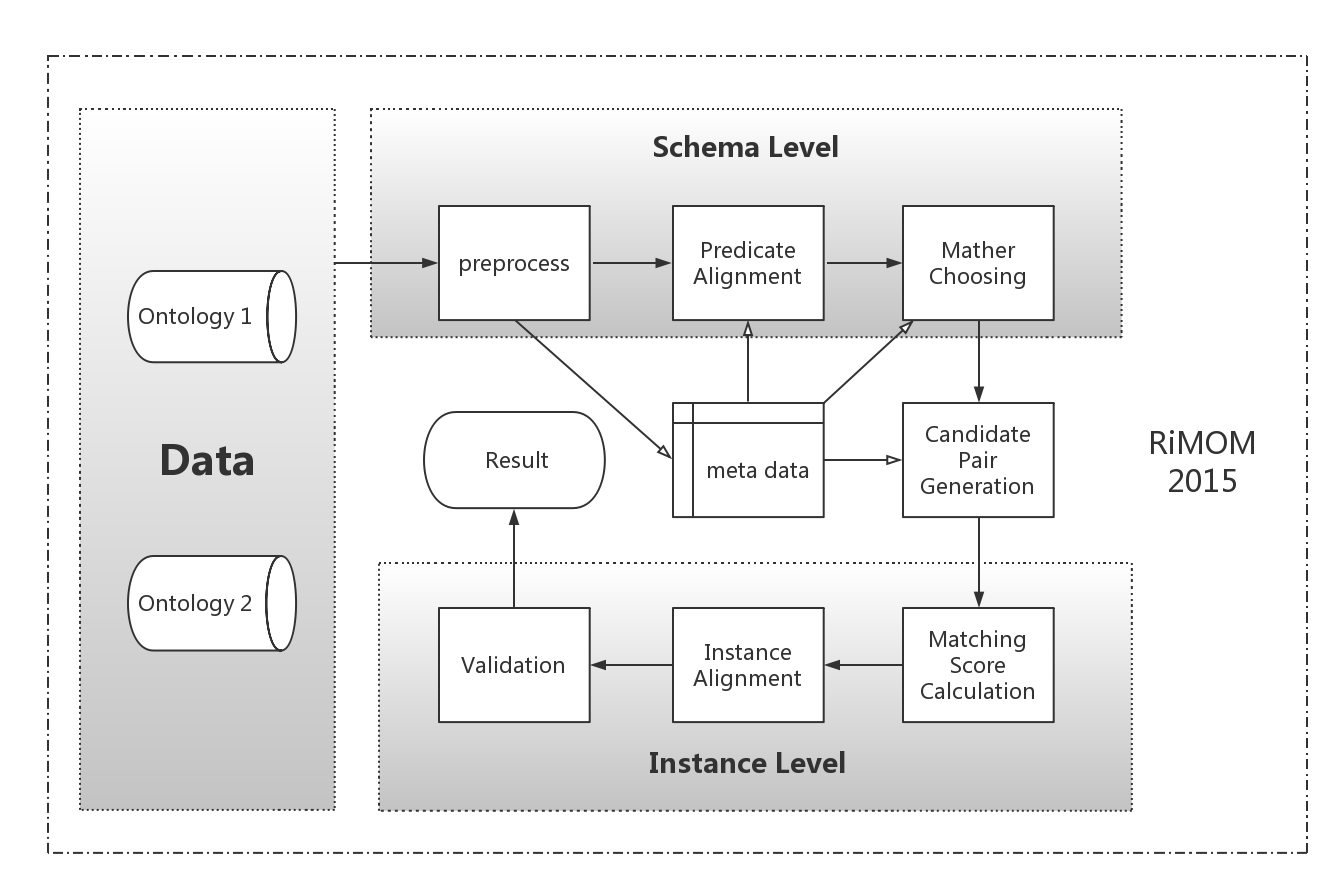
\includegraphics[width=0.8\textwidth]{./imagens/RiMOM_2015.png}
    \caption{Arquitetura do RiMOM-2015}
%	\footnotesize{Fonte: \cite{ferrara2008towards}2008towards}}
	\label{fig:rimom}
\end{figure}

\section*{LogMap}
Segundo \citeonline{jimenez2011logmap}, LogMap é uma solução para o alinhamento de ontologias. Logo, para dar suporte ao alinhamento de dados algumas alterações foram realizadas \cite{jimenez2015logmap}. Dentre as adaptações aplicadas está a adição de algoritmos de similaridade de texto.

o LogMap também utiliza índice invertido durante o processo de alinhamento. No entanto, o índice é gerado a partir das labels e de variações extraídas do WordNet ou do Unified Medical Language System (UMLS), com pode ser visto na Figura \ref{fig:logmap}. Além disso, raciocinadores como Hermit e Condor são utilizados para melhorar os resultados da indexação. 
Atualmente, existem três variações do LogMap, sendo elas LogMapC, LogMapBio e LogMapLt.  No primeiro, foi adicionado princípios de consistência e localidade, que são utilzados para melhorar a consistência dos alinhamentos. Essa variação foi desenvolvida com o objetivo de elevar a precisão dos alinhamentos apesar do decrescimento do recall. No segundo, foi utilizada uma extensão para o BioPortal, utilizando-o como um repositório de ontologias, permitindo que ontologias sejam recuperadas em tempo de execução. Por fim, mas não menos importante, se trata de uma versão “lightweight” do LogMap onde foi adicionado técnicas de similaridade de texto.

\begin{figure}[!ht]
	\centering
	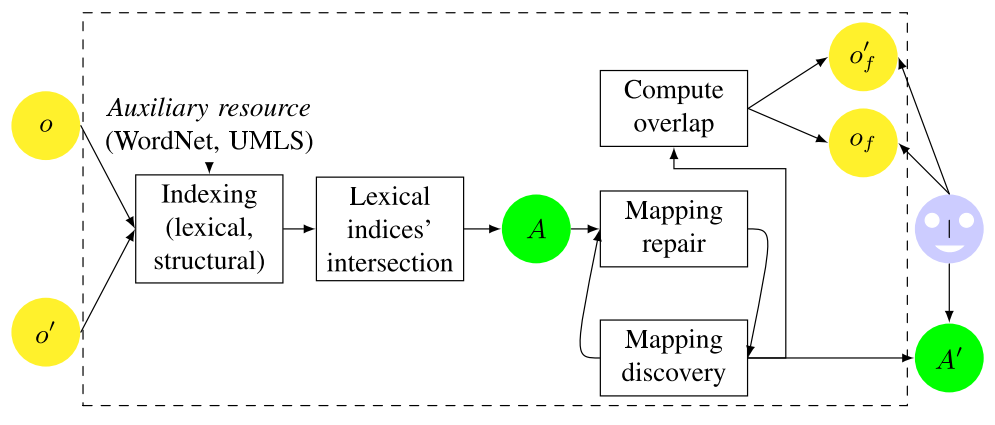
\includegraphics[width=0.8\textwidth]{./imagens/logmap.png}
    \caption{Arquitetura do LogMap}
	\footnotesize{Fonte: \cite{euzenat2013d}}
	\label{fig:logmap}
\end{figure}

\section*{Lily}
Desenvolvida durante o doutorado na Southeast University localizada em Nanjing no ano de 2008. Segundo  \citeonline{wang2015lily}, Lily se trata de uma solução para o alinhamento de ontologias, sendo composta por 5 estratégias principais, das quais apenas uma é dedicada ao alinhamento de dados.
o processo de alinhamento utilizado pelo Lily é composto pelo pré processamento, alinhamento e pós processamento (Figura \ref{fig:lily}).  A primeira etapa, consiste em analisar as ontologias de entrada para gerar metadados que serão utilizados para determinar parâmetros e estratégias. Na segunda, a ferramenta calcula a similaridade entre elementos de ontologias diferentes. Por fim, a etapa de pós processamento é responsável por exportar e refinar os alinhamentos gerados.

\begin{figure}[!ht]
	\centering
	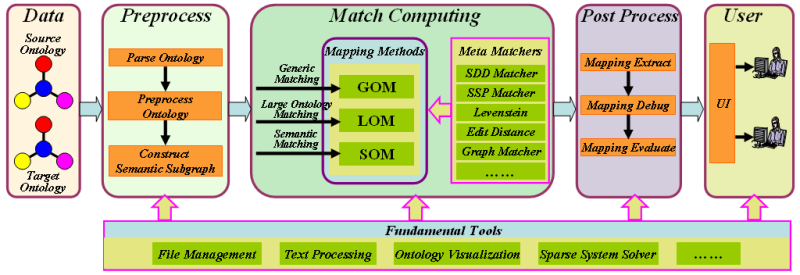
\includegraphics[width=0.9\textwidth]{./imagens/lily.png}
    \caption{Arquitetura do Lily}
	\footnotesize{Fonte: \cite{euzenat2013d}}
	\label{fig:lily}
\end{figure}

\section*{Comparação com a proposta}

Neste capítulo, algumas das principais ferramentas existentes foram apresentadas. Estas ferramentas tem o objetivo de alinhar dados conectados através através de diversas abordagens.
Dentre os sistemas apresentados, nenhum deles têm o alinhamento de dados como foco principal. Além disso, as abordagens apresentadas estão não permitem integração com soluções de armazenamento de triplas (Virtuoso, OWLim e outros), o que inviabiliza o seu uso em soluções mais complexas. Por fim, é descrito que as ferramentas são baseada em soluções de alinhamento de ontologias, porém a exploração no processo de alinhamento se limita à geração de metadados para auxiliar na escolha da estratégia que deve ser tomada. A tabela \ref{tab:comparacao} sumariza e compara os trabalhos relacionados com a proposta.

\begin{table}[h]
\centering
\caption{Comparação entre os trabalhos}
\label{tab:comparacao}
\begin{tabular}{@{}cccc@{}}
\toprule
Ferramenta & Integração a tripleStor & Suporte à ontologia & Foco               \\ \midrule
RiMOM-2015 &                         & X                   & Ontologia + Dados \\
LogMap     &                         & X                   & Ontologia + Dados \\
Lily       &                         & X                   & Ontologia + Dados \\
Proposta   & X                       & X                   & Dados             \\ \midrule
\end{tabular}
\end{table}
